\part{SW 13}
\section{Lernziele (Leitfragen)}
\begin{itemize}
    \item Was ist eine VPN? Wieso ist es «Virtual», wieso ist es «Private»?
    \item Was sind die Vorteile von VPNs im Vergleich zu traditionellen privaten Netzwerken?
    \item Was sind die Hauptarten von VPNs?
    \item Was sind die Hauptarten von Remote Access VPNs?
    \item Was ist IPSec? Was ist seine Verwendung?
    \item Woraus besteht eine IPSec Security Association?
    \item Was ist der Unterschied zwischen Transport und Tunnel Modi in IPSec?
    \item Was ist der Unterschied zwischen «Effectiveness» (Wirksamkeit) und «Efficiency» (Effizienz)?
    \item Was ist der Unterschied zwischen «Fault-tolerance» (Fehlertoleranz) und «Resiliency» (Resilienz)?
    \item Geben Sie Beispiele von Fehlertoleranz in Verbindung mit Netzwerktechnologien
    \item Geben Sie Beispiele von Resilienz in Verbindung mit Netzwerktechnologien
    \item Was ist Skalierbarkeit und wie wird es normalerweise erreicht?
    \item Beschreiben Sie zwei «Load Balancing» (Lastverteilung) Strategien
    \item Beschreiben Strategien um «single-points-of-failure» zu vermeiden
    \item Was sind die Hauptunterschiede zwischen 1G und gegenwärtigen Generationen (4G, 5G) von Mobilnetzwerke?
    \item Was ist die Verbindung zwischen IoT und Mobilnetzwerken (insbesondere 5G)?
    \item Warum werden nicht alle Mobilfunknetze auf den neuesten Standard aufgerüstet? Warum koexistieren verschiedene Mobilfunknetzgenerationen nebeneinander?
    \item Nennen Sie Beispiele für Anwendungsfälle von 5G-Netzen
    \item Nennen Sie Beispiele für die im IoT verwendeten Kommunikationstechnologien
    \item Nennen Sie Beispiele für die im IoT verwendeten Backend-Technologien
    \item Nennen Sie Beispiele für Anwendungsfälle von IoT
\end{itemize}

\section{Antworten}
\subsection*{Was ist eine VPN? Wieso ist es «Virtual», wieso ist es «Private»?}\index{VPN}
Virtual Private Network.
\begin{itemize}
    \item End-to-end: private Netzwerkverbindung über öffentliche Netzwerke
    \item Virtual: Informationen werden über öffentliches Netzwerk transportiert
    \item Private: Verkehr ist verschlüsselt um die Vertraulichkeit der Daten während dem Transport über dem öffentlichen Netzwerk zu wahren
\end{itemize}

\subsection*{Was sind die Vorteile von VPNs im Vergleich zu traditionellen privaten Netzwerken?}\index{VPN}
\begin{itemize}
    \item Kostensparend: Firmen können Kosten reduzieren und gleichzeitig Bandbreite erhöhen.
    \item Sicherheit: Verschlüsselungs- und Authentifizierungsprotokolle schützen Daten vor unbefugtem Zugriff
    \item Erweiterbarkeit: VPNs ermöglichen Firmen das Internet zu nutzen,
\end{itemize}

\subsection*{Was sind die Hauptarten von VPNs?}\index{{VPN!Hauptarten}}
\begin{itemize}
    \item Remote-access: dynamisch erstellt zwischen Client und VPN-Gateway
    \item Site-to-site: VPN-Gateways stellen eine ständige Verbindung her. Clients wissen nicht, dass im Hintergrund eine VPN existiert.
\end{itemize}

\subsection*{Was sind die Hauptarten von Remote Access VPNs?}\index{VPN!Hauptarten}
\begin{itemize}
    \item Clientless VPN Connection
    \item Client-based VPN connection
\end{itemize}

\subsection*{Was ist IPSec? Was ist seine Verwendung?}\index{IPsec}
IPSec ist ein IETF-Standard welcher definiert, wie VPN über IP-Netzwerke gesichert werden kann. IPSec schützt und authentisiert IP-Pakete zwischen Source und Destination und bietet essenzielle Sicherheitsfunktionen:
\begin{itemize}
    \item Vertraulichkeit (Confidentiality): nutzt Verschlüsselungsalgorithmen um zu verhindern, dass Inhalte von Datenpaketen auf dem Weg gelesen werden können
    \item Integrität (Integrity): nutzt Hashfunktionen um sicherzustellen, dass Pakete zwischen Source und Destination nicht geändert wurden
    \item Quell-Authentisierung: nutzt das Internet Key Exchange Protocol (IKE) um Source und Destination zu authentisieren
    \item Diffie-Hellmann: für sicheren Schlüsselaustausch
\end{itemize}

\subsection*{Woraus besteht eine IPSec Security Association?}\index{IPsec!Security Association}
\begin{figure}[H]
    \begin{center}
    \label{pic:SecurityAssociation}
    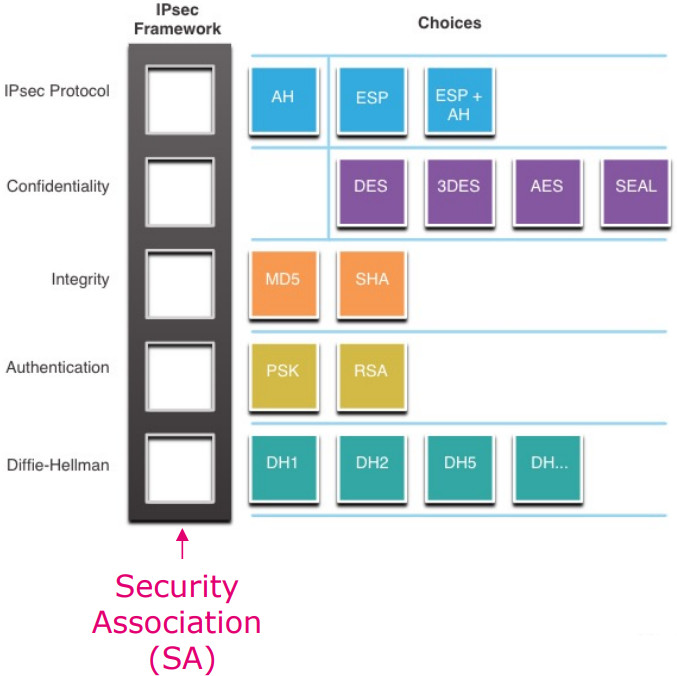
\includegraphics[width=\textwidth]{images/security_association.jpg}
    \caption{Security Association (\textsuperscript{\textcopyright}Cisco)}
    \end{center}
\end{figure}

\subsection*{Was ist der Unterschied zwischen Transport und Tunnel Modi in IPSec?}\index{IPsec!Modi}
Transport mode
\begin{itemize}
    \item Der IP-Header wird weder modifiziert noch verschlüsselt
    \item Inkompatibel mit NAT (authentisierter Inhalt)
    \begin{itemize}
        \item IP-Adresse kann nicht modifiziert werden
        \item Port-Nummern können nicht übersetzt werden
    \end{itemize}
\end{itemize}
\begin{figure}[H]
    \begin{center}
    \label{pic:IPsecTransportMode}
    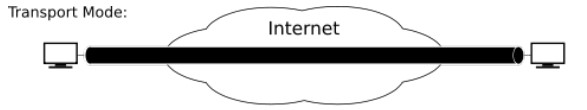
\includegraphics[width=\textwidth]{images/ipsec_transport_mode.jpg}
    \caption{IPsec Transport Mode}\cite{wiki}
    \end{center}
\end{figure}

Tunnel Mode
\begin{itemize}
    \item Gesamtes IP-Paket wird verschlüsselt und authentisiert
    \item Danach in ein neues IP-Paket gekapselt mit einem neuen IP-Header
    \item Verwendet um VPNs zu erstellen
    \item Kompatibel mit NAT
\end{itemize}
\begin{figure}[H]
    \begin{center}
    \label{pic:IPsecTunnelMode}
    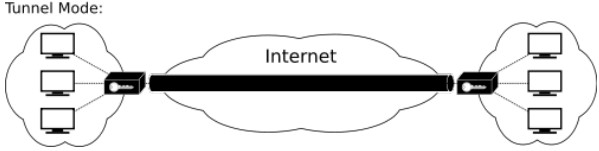
\includegraphics[width=\textwidth]{images/ipsec_tunnel_mode.jpg}
    \caption{IPsec Tunnel Mode}\cite{wiki}
    \end{center}
\end{figure}

\subsection*{Was ist der Unterschied zwischen «Effectiveness» (Wirksamkeit) und «Efficiency» (Effizienz)?}\index{Effectiveness}\index{Wirksamkeit}\index{Efficiency}
\begin{itemize}
    \item Effektivität: WAS. Was ist das Ergebnis? Etwas ist effektiv, wenn es zum Ergebnis führt.
    \item Effizienz: WIE. Wie kommt man zum Ergebnis? Etwas ist effizient, wenn man das Ziel wirtschaftlich erreicht, mit möglichst geringem Aufwand/Kosten.
\end{itemize}

\subsection*{Was ist der Unterschied zwischen «Fault-tolerance» (Fehlertoleranz) und «Resiliency» (Resilienz)?}\index{Fehlertoleranz}\index{Fault-Tolerance}\index{Resiliency}
\begin{itemize}
    \item Fault-tolerance: der Nutzer spürt von der Ausfallsicherung nichts
    \item Fault-resilience: es gibt eine kleine (merkbare) Periode, bei dem der Nutzer einen Unterbruch feststellen könnte
\end{itemize}

\subsection*{Geben Sie Beispiele von Fehlertoleranz in Verbindung mit Netzwerktechnologien}\index{Fehlertoleranz}\index{Fault-Tolerance}
Meshed Network, siehe \underline{\hyperref[sub:Topologies]{Topologien in Computernetzwerken}}, Seite \pageref{sub:Topologies}.

\subsection*{Geben Sie Beispiele von Resilienz in Verbindung mit Netzwerktechnologien}\index{Resiliency}
\begin{figure}[H]
    \begin{center}
    \label{pic:VirtualRouter}
    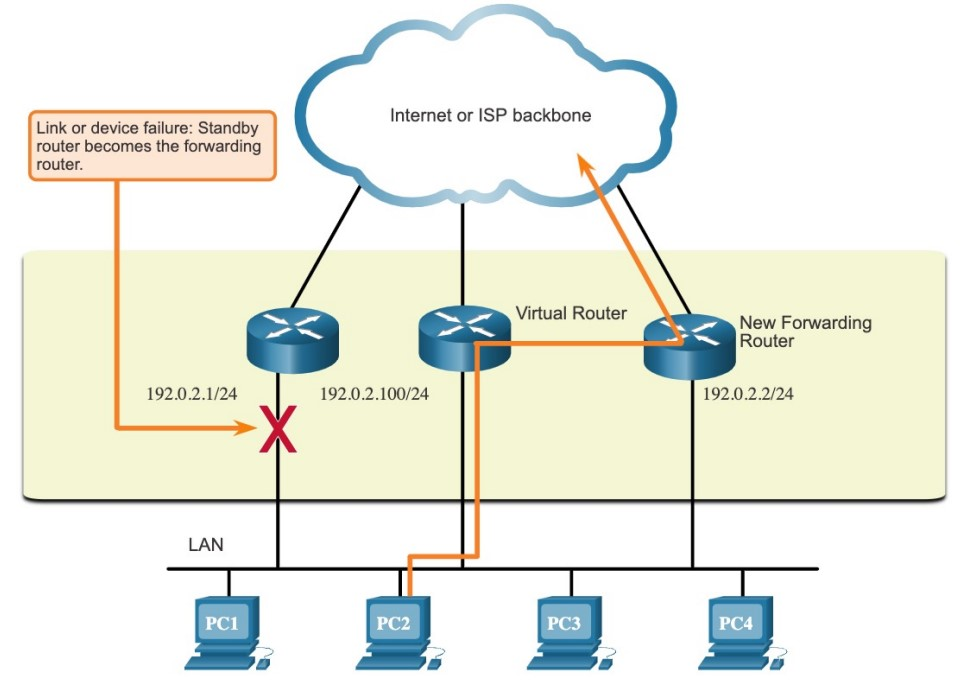
\includegraphics[width=\textwidth]{images/virtual_router.jpg}
    \caption{Virtual Router merkt Fehler und leitet zum anderen Router (\textsuperscript{\textcopyright}Cisco)}
    \end{center}
\end{figure}

\subsection*{Was ist Skalierbarkeit und wie wird es normalerweise erreicht?}\index{Scalability}
Siehe \underline{\hyperref[sub:NetworkScalability]{Skalierbarkeit im Netzwerk}}, Seite \pageref{sub:NetworkScalability} und dessen Abbildung \ref{pic:scalability}.

\subsection*{Beschreiben Sie zwei «Load Balancing» (Lastverteilung) Strategien}\index{Load Balancing}
\begin{itemize}
    \item Round-Robin
    \begin{itemize}
        \item Sind beispielsweise mehrere Server mit derselben Aufgabe betraut, wird für jede Abfrage der nächste Server aufgerufen.
    \end{itemize}
    \item Lastabfrage
    \begin{itemize}
        \item Dies bietet den Vorteil gegenüber dem Round-Robin, dass der Lastzustand der Server bekannt ist und die Anfrage zu dem Server weitergereicht wird, welcher die geringste Auslastung hat.
    \end{itemize}
\end{itemize}

\subsection*{Beschreiben Strategien um «single-points-of-failure» zu vermeiden}\index{Single Point of Failure}
Es gibt immer irgendwo ein Flaschenhals. Man kann zwar zwei Gateways betreiben, aber was, wenn der Load-Balancer ausfällt? Man kann das Risiko eines Ausfalles zwar vermindern, aber zu 100 \% schützen kann man nicht. Jedoch versucht man mit Redundanzen dies zu Umgehen. Beispielsweise hat man seine Daten auf 2 standortunabhängige Servercenter. Aber wenn in der Firma der Strom ausfällt, nützen auch zwei Servercenter nichts.

\subsection*{Was sind die Hauptunterschiede zwischen 1G und gegenwärtigen Generationen (4G, 5G) von Mobilnetzwerke?}\index{Mobilnetzwerke}
5G hat viel viel mehr Antennen als 1 G. Dadurch kann die Sendeleistung von 5G reduziert werden (Elektrosmog), jedoch ist die Verbindung um einiges stärker und hat grosse Senderaten.

\subsection*{Was ist die Verbindung zwischen IoT und Mobilnetzwerken (insbesondere 5G)?}\index{IoT}\index{Mobilnetzwerke}
\begin{itemize}
    \item Telemedizin - Chirurg der eine Operation in den USA aus der Schweiz macht
    \item Verbindung MUSS STABIL SEIN
    \item Deswegen braucht es starke Mobilnetze
    \item Autonome verbundene Autos müssen effizient und zuverlässig miteinander kommunizieren können
\end{itemize}


\subsection*{Warum werden nicht alle Mobilfunknetze auf den neuesten Standard aufgerüstet? Warum koexistieren verschiedene Mobilfunknetzgenerationen nebeneinander?}\index{Mobilnetzwerke}
Ältere Technologien dienen als Backups. Es wird zwar ausgebaut, doch spielen auch die Kosten eine Rolle.

\subsection*{Nennen Sie Beispiele für Anwendungsfälle von 5G-Netzen}\index{Mobilnetzwerke}
\begin{itemize}
    \item Augmented reality
    \item Remote Collaboration
    \item Immersive Gaming
\end{itemize}

\subsection*{Nennen Sie Beispiele für die im IoT verwendeten Kommunikationstechnologien}\index{IoT}\index{Mobilnetzwerke}
\begin{itemize}
    \item Full Duplex
    \begin{itemize}
        \item Senden und Daten gleichzeitig empfangen
    \end{itemize}
    \item Master Slave Verbindungen (Half duplex)
\end{itemize}

\subsection*{Nennen Sie Beispiele für die im IoT verwendeten Backend-Technologien}\index{IoT!Technologien}
\begin{itemize}
    \item JavaScript
    \item Python
    \item PHP
    \item .NET
\end{itemize}

\subsection*{Nennen Sie Beispiele für Anwendungsfälle von IoT}\index{IoT!Anwendungsfälle}
\begin{itemize}
    \item Toilette mit Internetanbindung (warum auch immer)
    \item Lampen (Haussteuerung)
    \item Staubsauger
    \item Autos
\end{itemize}
